\documentclass{article}
\usepackage{fullpage}
\usepackage{graphicx,color}

\usepackage{amssymb}
\usepackage{braket}
\usepackage{physics}
\usepackage{qcircuit}


\title{Symbolic Retrodictive Execution of Quantum Circuits}
\author{Jacques Carette \qquad Gerardo Ortiz \qquad Amr Sabry}
\begin{document}
\maketitle

\begin{abstract}
The quantum circuit model consists of two classes of gates: (i) quantum counterparts to classical reversible gates (e.g., Toffoli gates), and (ii) genuine quantum gates with no classical counterpart (e.g., Hadamard and phase gates). We make the remarkable observation, that, for a number of quantum algorithms, judicious reasoning about the classical components, ignoring all the quantum gates, is sufficient. Put differently, in those cases, the quantum gates serve no fundamental purpose and are actually distracting from an underlying efficient classical algorithm. The result relies on the ability to symbolically execute circuits, especially in a retrodictive fashion, i.e., by making partial observations at the output site and proceeding backwards to infer the implied initial conditions.
\end{abstract}

%%%%%%%%%%%%%%%%%%%%%%%%%%%%%%%%%%%%%%%%%%%%%%%%%%%%%%%%%%%%%%%%%%%%%%%%%%%%%%%%%%%%%%%%%%%%%%%%%%%%%%%%%%%%%%%%%%%%%
\section{Introduction}

% Just dumping the points from today's discussion here
\begin{itemize}
\item Retrodictive execution more efficient in some cases. What cases?
\item Here are three examples: Deutsch-Jozsa, Simon, Shor when period is close to a power of 2
\item Symbolic (retrodictive) evaluation as a broader perspective to classical computation
\item Symbolic execution allows you to express/discover interference via shared variables
\item When interference pattern is simple symbolic execution reveals solutions faster (and completely classically) 
\item Symbolic execution as a “classical waves” computing paradigm
\end{itemize}

%%%%%%%%%%%%%%%%%%%%%%%%%%%%%%%%%%%%%%%%%%%%%%%%%%%%%%%%%%%%%%%%%%%%%%%%%%%%%%%%%%%%%%%%%%%%%%%%%%%%%%%%%%%%%%%%%%%%%
\section{A Complete Example}

Consider the small circuit in Fig.~\ref{fig:factor}. The scenario we are investigating is the following. The initial state of $c_2,c_1,c_0$ is unknown but both the initial state and final state of $q_1,q_0$ are known. The initial state is clearly $00$ and let's assume for the remaining of this example that the final state is $01$. The question is what can we infer about $c_2,c_1,c_0$? To answer the question, we will symbolically evaluate the circuit starting from the final state $c_0,c_1,c_2,1,0$ and going backwards towards the initial state as shown in Fig.~\ref{fig:deriv}. In step (1), we encounter a \texttt{cx} acting on $q_1$ and $q_0$ which are known. In step (2), we are not so lucky: we encounter a \texttt{ccx} gate with one unknown control wire but all hope is not lost. The action of $\texttt{ccx}~a~b~c$ is to update $c$ to be $a \wedge b \oplus c$ where $\wedge$ is boolean conjunction (often omitted when clear from context) and $\oplus$ is the exclusive-or operation. In step (2), this means that the target wire $q_1$ should be updated to $1 \wedge c_0 \oplus 0$ which simplifies to $c_0$. 

At the end of the retrodictive execution, we conclude that $q_0 = 1 \oplus c_0 \oplus c_1$ and $q_1 = c_0 \oplus c_2$ which needs to reconciled with the initial condition that $q_0 = q_1 = 0$. Solving these equations gives two possible solutions for $c_2j,c_1,c_0$: either $c_2,c_1,c_0 = 010$ or $c_2,c_1,c_0 = 101$.

Another perspective on this analysis is the following. Assume $c_2,c_1,c_0$ started in an equal superposition and that $q_1,q_0$ were measured to be $01$ after applying the circuit to the incoming superposition. The measurement of $q_1q_0$ would essentially cause a \emph{phase kickback} collapsing the equal superposition of all possible values of $c_2,c_1,c_0$ to just the two possible values that are consistent with the measurement. 

\begin{figure}[t]
\[\begin{array}{lclr}
&& c_0~c_1~c_2~(q_0=1)~(q_1=0) & (0) \\
(\texttt{cx}~q_1~q_0)      \\ && c_0~c_1~c_2~(q_0=1)~(q_1=0) & (1) \\
(\texttt{ccx}~c_0~q_0~q_1) \\ && c_0~c_1~c_2~(q_0=1)~(q_1=c_0) & (2) \\
(\texttt{cx}~q_1~q_0)      \\ && c_0~c_1~c_2~(q_0=1 \oplus c_0)~(q_1=c_0) & (3) \\
(\texttt{x}~q_1)           \\ && c_0~c_1~c_2~(q_0=1 \oplus c_0)~(q_1=1 \oplus c_0) & (4) \\
(\texttt{ccx}~c_0~q_1~q_0) \\ && c_0~c_1~c_2~(q_0=1 \oplus c_0)~(q_1=1 \oplus c_0) & (5) \\
(\texttt{x}~q_1)           \\ && c_0~c_1~c_2~(q_0=1 \oplus c_0)~(q_1=c_0) & (6) \\
(\texttt{cx}~q_1~q_0)      \\ && c_0~c_1~c_2~(q_0=1)~(q_1=c_0) & (7) \\
(\texttt{ccx}~c_1~q_0~q_1) \\ && c_0~c_1~c_2~(q_0=1)~(q_1=c_0 \oplus c_1) & (8) \\
(\texttt{cx}~q_1~q_0)      \\ && c_0~c_1~c_2~(q_0=1 \oplus c_0 \oplus c_1)~(q_1=c_0 \oplus c_1) & (9) \\
(\texttt{cx}~c_1~q_1)      \\ && c_0~c_1~c_2~(q_0=1 \oplus c_0 \oplus c_1)~(q_1=c_0) & (10) \\
(\texttt{cx}~c_2~q_1)      \\ && c_0~c_1~c_2~(q_0=1 \oplus c_0 \oplus c_1)~(q_1=c_0 \oplus c_2) & (11)
\end{array}\]
\caption{Retrodictive execution of the circuit in Fig.~\ref{fig:factor}}
\label{fig:deriv}
\end{figure}

\begin{figure}[t]
    \centering
    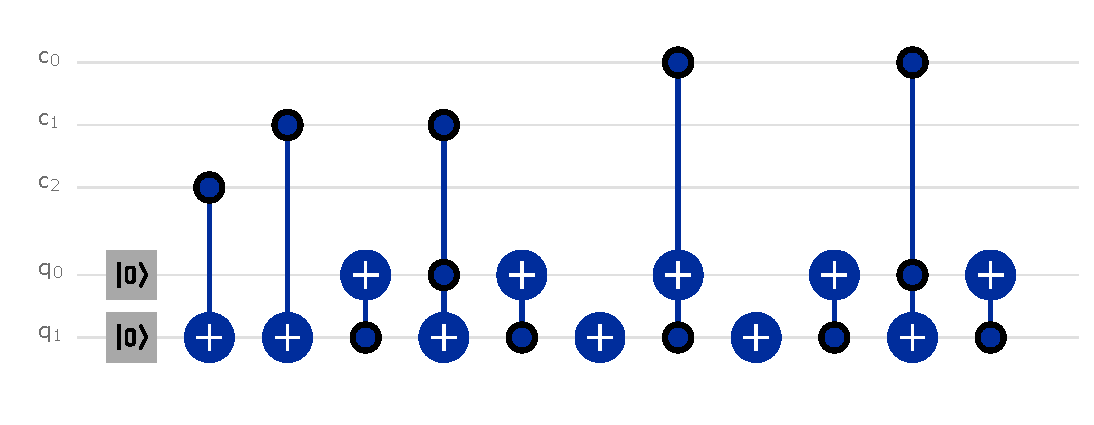
\includegraphics[scale=0.7]{factor.pdf}
    \caption{A small example circuit}
    \label{fig:factor}
\end{figure}

Fig.~\ref{fig:adder} shows a larger circuit. The top five wires are the interesting inputs while the bottom five wires serve as ancilla bits initialized to fixed values. The question we are interested in this case is the following: say we learn that at the end of the execution we have $b_2b_1b_0 = 001$, what possible input values for $a_1a_0$ and $b_2b_1b_0$ could have produced such a result? Using the same process as above, we calculate $b_0 = 1 \oplus a_0 \oplus a_1$, $b_1 = a_1 \oplus a_0a_1$, and $b_2 = 0$.

\begin{figure}[t]
    \centering
    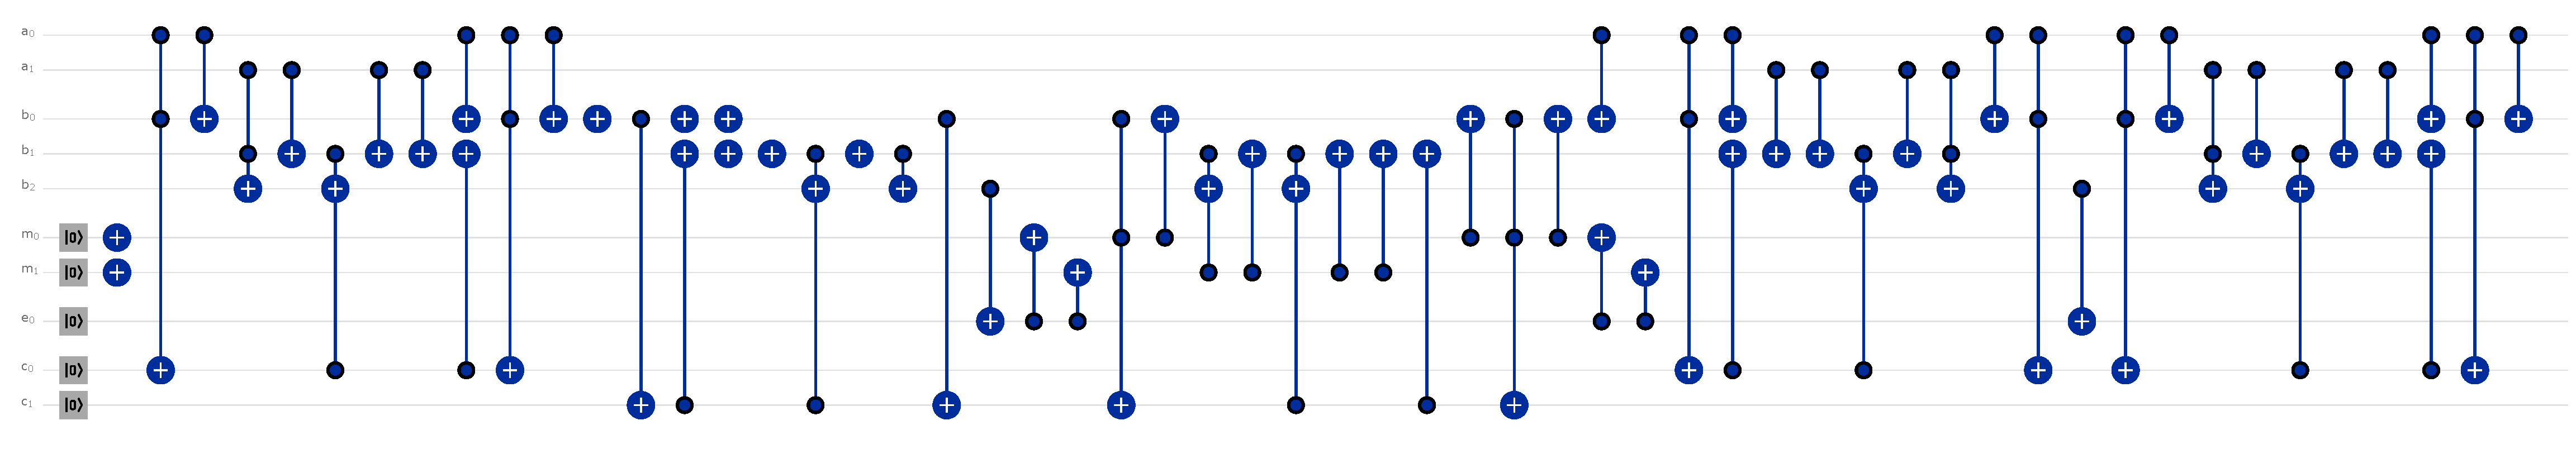
\includegraphics[scale=0.2]{adder.pdf}
    \caption{A larger example circuit}
    \label{fig:adder}
\end{figure}



Quantum algorithms typically operate on a \emph{black box} holding a classical function whose properties need to be computed. The general structure of these algorithms is to (i) create a superposition of values to be passed as inputs to the black box, (ii) apply the operation inside the black box, and (iii) post-process the output of the black box. We observe that, in quite a few cases, steps (i) and (iii) are actually unnecessary and that the entire ``quantum'' algorithm can be executed by forward or backward, full or partial, efficient classical \emph{symbolic execution} of the black box. 


typical use: superposition, Uf, measure second register; we only care about which x has f(x) = r

%%%%%%%%%%%%%%%%%%%%%%%%%%%%%%%%%%%%%%%%%%%%%%%%%%%%%%%%%%%%%%%%%%%%%%%%%%%%%%%%%%%%%%%%%%%%%%%%%%%%%%%%%%%%%%%%%%%%%
\section{Retrodictive Execution: Taking advantage of the future}

We need to explain ideas about time-reversal, prediction and retrodiction in 
physics. The laws of computation and the laws of physics are intimately related. 
When does knowing something about the future help us unveil the structure or 
symmetries of the past? It is like a detective story, but one with 
ramifications in complexity and/or efficiency. Problems involving questions 
where answers demand a Many(past)-to-one(future) map are at the root of 
our proposal.... {\color{red} Difference between exploiting or not entanglement
in the unitary evolution.}

%%%%%%%%%%%%%%%%%%%%%%%%%%%%%%%%%%%%%%%%%%%%%%%%%%%%%%%%%%%%%%%%%%%%%%%%%%%%%%%%%%%%%%%%%%%%%%%%%%%%%%%%%%%%%%%%%%%%%
\section{Partial Symbolic Evaluation with Algebraic Normal Form (ANF)}

We should use two prototypical examples to illustrate main ideas before going to the 
complex ones. The examples I have in mind are: Deutsch-Josza and Simon (precursor 
of Shor's). There are prior works on de-quantization of the first problem and should 
make contact with their resolution. Perhaps we can show that they are as 
efficient classically? That would justify retrodiction alone. The more complex 
(and important) case of factorization should be the natural follow up. 

The idea of symbolic execution is not tied to forward or backward execution. We should introduce it in a way that is independent of the direction of execution. What the idea depends on however is that the wave function, at least in the cases we are considering, can be represented as equations over booleans. 

Wave Functions as Equations over Booleans

in the typical scenario for using quantum oracles, we can represent wave function as equations over booleans; equations represent the wave function but the solution is unobservable just like the components of the superposition in the wave function are not observable; just like we don't directly get access to the components of the wave function; we don't directly get access to the solution of the equations; need to "observe" the equations

we can go backwards with an equation (representing a wave function sigma x where f(x) = r and go back towards the present to calculate the wave function (represented as equations again) 

Musing: how to explain complementarity when wave function is represented as an equation? Kochen specker;
 
or contextuality
 
observer 1 measures wires a,b; obs2 measures wires b,c; not commuting; each obs gives partial solution to equations; but partial solutions cannot lead to a global solution
 
KS suggests that equations do not have unique solutions; only materialize when you measure;

can associate a probability with each variable in a equation: look at all solutions and see the contribution of each variable to these solutions. 

%%%%%%%%%%%%%%%%%%%%%%%%%%%%%%%%%%%%%%%%%%%%%%%%%%%%%%%%%%%%%%%%%%%%%%%%%%%%%%%%%%%%%%%%%%%%%%%%%%%%%%%%%%%%%%%%%%%%%
\section{Classical Algorithms from Quantum Circuits}

%%%
\subsection{Deutsch}

The problem is to determine if a function $\mathbb{B} \rightarrow \mathbb{B}$ is constant or balanced. Here is the circuit for the Deutsch algorithm after removing all the quantum gates:

\begin{equation}\label{eq:deutsch}
  \Qcircuit @C=1em @R=.7em {
   \lstick{x} & \multigate{1}{U_f} & \rstick{x} \qw \\
   \lstick{y} & \ghost{U_f}        & \rstick{\ket{0}} \qw
  }
\end{equation}
\medskip 

 We fix the ancillary output to a possible boundary condition, say $\ket{0}$, and perform a retrodictive execution of the circuit. This execution produces a formula for $y$ that depends on the function $f$ in the black box. When the function $f$ is a constant function, the formula is the corresponding constant $0$ or $1$. When the function is balanced the resulting formula is $x$ (when the function is the identity) or $1+x$ (when the function is boolean negation). 

%%%
\subsection{Deutsch-Jozsa}

The problem is a generalization of the previous one: the question is to determine if a function  $\mathbb{B}^n \rightarrow \mathbb{B}$ is constant or balanced. The circuit is identical to above except that $x$ is now a collection of qubits:

\begin{equation}\label{eq:deutsch-jozsa}
  \Qcircuit @C=1em @R=.7em {
   \lstick{x_0}     & \multigate{4}{U_f} & \rstick{x_0}     \qw \\
   \lstick{x_1}     & \ghost{U_f}        & \rstick{x_1}     \qw \\
   \lstick{\ldots}  & \ghost{U_f}        & \rstick{\ldots}  \qw \\
   \lstick{x_{{n-1}}} & \ghost{U_f}        & \rstick{x_{{n-1}}} \qw \\
   \lstick{y}       & \ghost{U_f}        & \rstick{\ket{0}} \qw
  }
\end{equation}
\medskip 

Again, we fix the ancillary output to a possible boundary condition, say $\ket{0}$, and perform a retrodictive execution of the circuit. This execution produces a formula for $y$ that depends on the function $f$ in the black box. When the function $f$ is a constant function, the formula is the corresponding constant $0$ or $1$. When the function is balanced the resulting formula involves at least one variable $x_i$. 

%%%
\subsection{Bernstein-Vazirani}

We are given a function $f_s : \mathbb{B}^n \rightarrow \mathbb{B}$ that hides a string $s \in \mathbb{B}^n$. We are promised the function is defined as:
\[
f_s (x) = \sum_{i=0}^{n-1} s_ix_i \quad \mod{2}
\]
and the goal is to determine $s$.  

The circuit below demonstrates the situation when  $n=8$ and the hidden string $s = 00111010$:

\begin{equation}\label{eq:bernstein-vazirani}
  \Qcircuit @C=1em @R=.7em {
   \lstick{x_0} & \qw      & \qw      & \qw       & \qw       & \rstick{x_0}     \qw \\
   \lstick{x_1} & \ctrl{7} & \qw      & \qw       & \qw       & \rstick{x_1}     \qw \\
   \lstick{x_2} & \qw      & \qw      & \qw       & \qw       & \rstick{x_2}     \qw \\
   \lstick{x_3} & \qw      & \ctrl{5} & \qw       & \qw       & \rstick{x_3}     \qw \\
   \lstick{x_4} & \qw      & \qw      & \ctrl{4}  & \qw       & \rstick{x_4}     \qw \\
   \lstick{x_5} & \qw      & \qw      & \qw       & \ctrl{3}  & \rstick{x_5}     \qw \\
   \lstick{x_6} & \qw      & \qw      & \qw       & \qw       & \rstick{x_6}     \qw \\
   \lstick{x_7} & \qw      & \qw      & \qw       & \qw       & \rstick{x_7}     \qw \\
   \lstick{y}   & \targ    & \targ    & \targ     & \targ     & \rstick{\ket{0}} \qw
  }
\end{equation}
\medskip 

Symbolically running the circuit in a retrodictive fashion reveals that $y = x_1 \oplus x_3 \oplus x_4 \oplus x_5$ which are exactly the bits that are equal to 1 in the hidden string. 

%%%
\subsection{Simon}

We are given a 2-1 function $f : \mathbb{B}^n \rightarrow \mathbb{B}^n$ where there exists an $a$ such $f(x) = f(x \oplus a)$ for all $x$; the goal is to determine $a$. 

The circuit below demonstrates the situation when $n=2$ and $a = 3$. 

\begin{equation}\label{eq:simon}
  \Qcircuit @C=1em @R=.7em {
   \lstick{x_0} & \ctrl{2} & \ctrl{3} & \qw      & \qw      & \rstick{x_0} \qw \\
   \lstick{x_1} & \qw      & \qw      & \ctrl{1} & \ctrl{2} & \rstick{x_1} \qw \\
   \lstick{a_0} & \targ    & \qw      & \targ    & \qw      & \rstick{a_0} \qw \\
   \lstick{a_1} & \qw      & \targ    & \qw      & \targ    & \rstick{a_1} \qw 
  }
\end{equation}
\medskip 

The circuit implements the black box $U_f (x,a) = (x, f(x) \oplus a)$. We first pick a random $x$, say $x = 3$, fix the initial condition $a = 0$ and run the circuit forward. This execution produces, in the second register, the value of $f(x) = 0$. We now run a symbolic retrodictive execution with $a = 0$ at the output site. That execution produces information on all values of $a$ that are consistent with the observed result. In this case, we get: $a_0 = x_0 + x_1$ and $a_1 = x_0 + x_1$. In other words, when $x_0=x_1$, we have $a=0$, and when $x_0 \neq x_1$, we have $a=3$ which is indeed the desired hidden value. 

%%%%%%%%%%%%%%%%%%%%%%%%%%%%%%%%%%%%%%%%%%%%%%%%%%%%%%%%%%%%%%%%%%%%%%%%%%%%%%%%%%%%%%%%%%%%%%%%%%%%%%%%%%%%%%%%%%%%%
\section{Complexity Analysis}

one pass over circuit BUT complexity of normalizing to ANF not trivial; be careful

%%%%%%%%%%%%%%%%%%%%%%%%%%%%%%%%%%%%%%%%%%%%%%%%%%%%%%%%%%%%%%%%%%%%%%%%%%%%%%%%%%%%%%%%%%%%%%%%%%%%%%%%%%%%%%%%%%%%%
\section{Conclusion}

%%%%%%%%%%%%%%%%%%%%%%%%%%%%%%%%%%%%%%%%%%%%%%%%%%%%%%%%%%%%%%%%%%%%%%%%%%%%%%%%%%%%%%%%%%%%%%%%%%%%%%%%%%%%%%%%%%%%%
%%%%%%%%%%%%%%%%%%%%%%%%%%%%%%%%%%%%%%%%%%%%%%%%%%%%%%%%%%%%%%%%%%%%%%%%%%%%%%%%%%%%%%%%%%%%%%%%%%%%%%%%%%%%%%%%%%%%%

\end{document}